\section{Concept}\label{sec:konzept}
Based on the survey, a concept for a voice assistant was developed. The costs for needed resources were neglected. An important requirement of the concept is data protection. The design principles for the multi-sided security of data according to Kai Rannenberg puts the following four points in the foreground \cite{kairannenberg}:

\begin{enumerate}
	\item Data Minimization
	\item Control options for the user 
	\item Choices and negotiation options 
	\item Decentralization and Distribution
\end{enumerate} 

As part of this concept, the focus is on the first three points. Often, applications capture data from a user that is not used to improve applications but to analyze users and resell them. Therefore, the concept should ensure that an application only obtains data from users who really need it. Furthermore, the collected data should be presented transparently to the users. Thus, users can also manipulate or anonymize their collected data.

This results in the following requirements for the language assistant to be developed:
\begin{itemize}
	\item User-Controlled-Privacy
	\item Functionality
	\item Performance
	\item User Friendliness	
\end{itemize}

User-Controlled Privacy allows a user to determine what data they share with them for specific applications. However, applications also require a user's data to provide usability. An example is the question of a language assistant according to the weather forecast. If the voice assistant knows where a user is currently located, he can provide the weather forecast for the current position of the user. Otherwise, the language assistant would first have to ask the user for which location to give him a weather forecast. If a user does not want to share his data with an application, he can set a fictitious context. This allows the user to use the applications, but at the expense of user-friendliness.

A context describes the properties of a user and is very extensive, as shown in Figure \ref{fig:context}. Examples include the cultural background, one's own interests and hobbies, as well as the social environment.

\begin{figure}[!h]
	\centering
	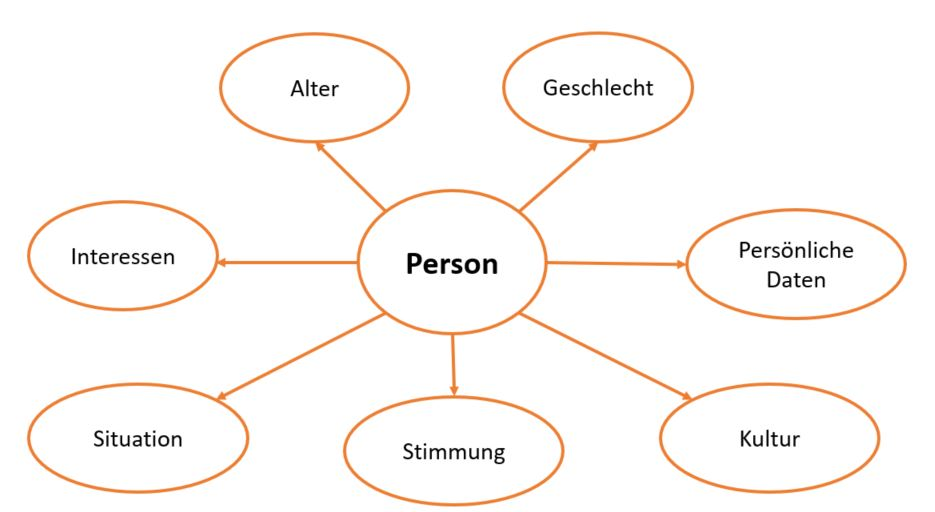
\includegraphics[width=1\linewidth]{Picture/Kontext}
	\caption[User Context]{User Context}
	\label{fig:context}
\end{figure}





